\documentclass[a4paper,12pt]{article}

\usepackage{geometry}       % Required for page layout.
\usepackage{hyperref}       % Required for hyperlinks.
\usepackage{graphicx}       % Required for figures.
\usepackage{subfig}         % Required for minipages.
% \usepackage{caption}
% \usepackage{subcaption}
\usepackage{placeins}
\usepackage{float}

\usepackage{amsmath}

\newgeometry{vmargin={25.4mm}, hmargin={27mm,27mm}}
\setlength\parindent{0pt}   % Disable paragraph indent.

\title{Final Project: Polymers as 3D Random Walks}
\author{
  Elias Rilegård\\
  \texttt{eliasril@kth.se}
}

\begin{document}
\maketitle

\section*{Introduction}

In the 2nd project of this course, we analyzed and discussed how organic polymers can be approximated and simulated
using 2D random walks. However, like everything else in the world, polymers are three-dimensional. This final
project builds on top of Project 2, by simulating the polymers as 3D random walks instead of 2D. The goal of this
project is to analyze fundamental changes of how simulating a polymer with random walks changes when stepping up
from two dimensions into three. Comparisons will be made not only between the different ways to simulate polymers
in 3D, but also against the 2D case. This report will also roughly follow the structure of the questions given in
Project 2.

% rip 2d grid walks from project 2
% do 2d chain walks

% step up into 3d, grid and chain walks
% notice how to generate vector with uniform spherical distribution
% RMSD and RMSF, (any difference to the 2d case) any difference between styles of walks?
% SEE?
% Self avoiding case
% does sphere radius affect RMSD and RMSF?
% comparison between non and self avoiding walk? any major differences? optimizations in generating walk?

% Compare RMSD between non and self avoiding walks?

\section*{Simple 2D Random Walks}

To begin, we will stay in two dimensions. Writing a program that generates 2D random walks with unit step length
either along a grid or as a freely jointed chain by taking a unit step in a random angle, and then graphing the
generated walks, yields the following.

\begin{figure}[!ht]
  \centering
  \begin{minipage}{0.49\textwidth}
    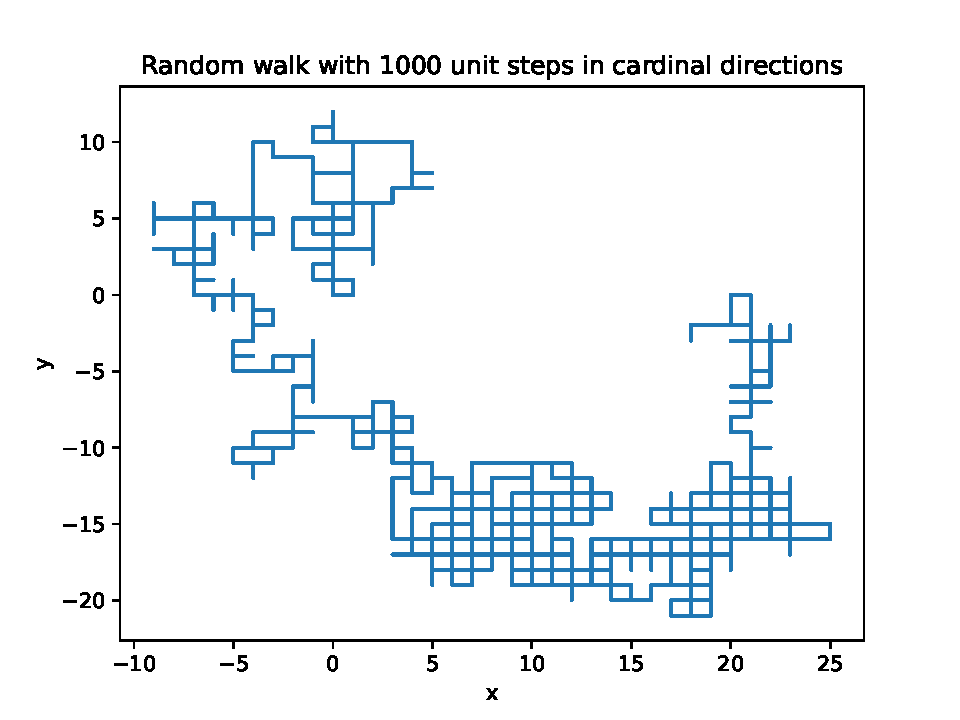
\includegraphics[width=\textwidth]{img/0-grid-1000.pdf}
  \end{minipage}
  \begin{minipage}{0.49\textwidth}
    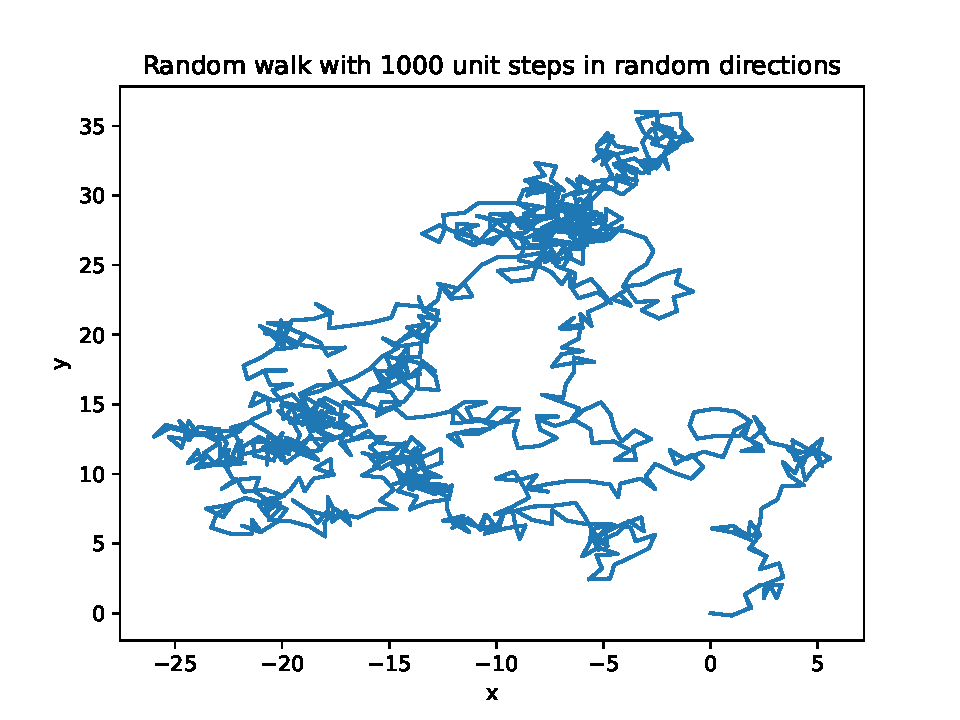
\includegraphics[width=\textwidth]{img/0-chain-1000.pdf}
  \end{minipage}
\end{figure}

2D random walks are further discussed in Project 2.

\section*{Uniform Angle Distributions}

A large portion of this project revolves around freely jointed chains (a chain with fixed length links, but with
random orientations), since they in theory can describe a polymer in a much more accurate way, due to not being
limited to sharp $90^{\circ}$ angle turns. A major component of the simulation of freely jointed chains is the
uniform distribution of angles used when building the random walk.

\subsection*{Two Dimensions}

In the two dimensional case, we can generate a unit vector by using polar coordinates, setting the radius $r = 1$
and generating a random value $\theta \in [0, 2\pi]$. We can then calculate the $x$ and $y$ components of the
vector by taking $\cos \theta$ and $\sin \theta$ respectively.

\subsection*{Three Dimensions}

Moving up to three dimensions, we \emph{don't} want to use spherical coordinates (Where $\theta \in [0, 2\pi)$,
$\phi \in [0, \pi]$) to generate a random vector, since that results in an incorrect distribution. MathWorld
provides an excellent explanation as to why: It happens due to the fact that the area element

\begin{equation*}
  \mathrm{d}\Omega = \sin \phi \, \mathrm{d} \theta \, \mathrm{d} \phi
\end{equation*}

is a function of $\phi$, meaning points picked with this particular method will be more concentrated towards the
poles of the corresponding unit sphere from which we are sampling. To generate points which are correctly
distributed, we need to use an equal-area projection of the surface of a sphere to a rectangle. Most papers
recommend choosing variables $u,\, v$ being uniformely distributed over $[0, 1]$. We can calculate

\begin{equation*}
  \begin{aligned}
    \theta &= 2 \pi u \\
    \phi &= \arccos(2 v - 1)
  \end{aligned}
\end{equation*}

to obtain the angles used for spherical coordinates to describe the set of points which are uniformely distributed
on the surface of a sphere with a given radius. The area element described above can also be expressed as

\begin{equation*}
  \mathrm{d} \Omega = \sin \phi\, \mathrm{d} \theta\, \mathrm{d} \phi = -\mathrm{d} \theta\, \mathrm{d} (\cos \phi)
\end{equation*}

and to save ourselves unnecessary computations in the long run (since we'd have to compute the sine and cosine of
these angles), we can instead let $u = \cos \phi$ be uniformely distributed over $[-1,\, 1$], which gives
$\mathrm{d}u = \sin \phi \, \mathrm{d} \phi$. We can then calculate the points

\begin{equation*}
  \begin{aligned}
    x &= \sqrt{1 - u^2} \, \cos \theta \\
    y &= \sqrt{1 - u^2} \, \sin \theta \\
    z &= u
  \end{aligned}
\end{equation*}

with $\theta \in [0, 2 \pi)$ and $u \in [-1,\, 1]$.\footnote{Whether or not the bounds of the interval are included
or not is irrelevant since the probability of generating a single random number with any specific value is zero.
In the code, the bounds are \emph{not} included as a consequence of how Python's \texttt{random.random()} function
works.} This is the algorithm we will use to generate random unit vectors. \cite{MathWorld}

\section*{Simple 3D Random Walks}

Moving up to three dimensions, visualizing the paths become a little tricker due to projection issues becoming
relevant, but the perspectives chosen should still retain as much information as possible in regards to the path's
actual shape. Samples from the generated grid paths looks like the following.

\begin{figure}[!ht]
  \centering
  \begin{minipage}{0.49\textwidth}
    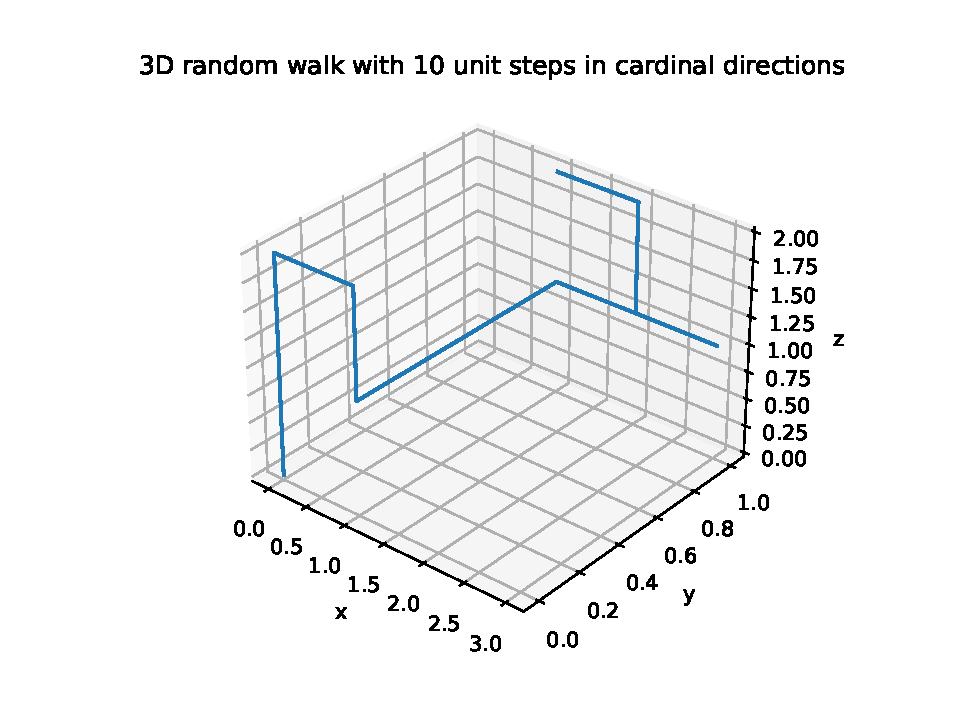
\includegraphics[width=\textwidth]{img/1-grid-10.pdf}
  \end{minipage}
  \begin{minipage}{0.49\textwidth}
    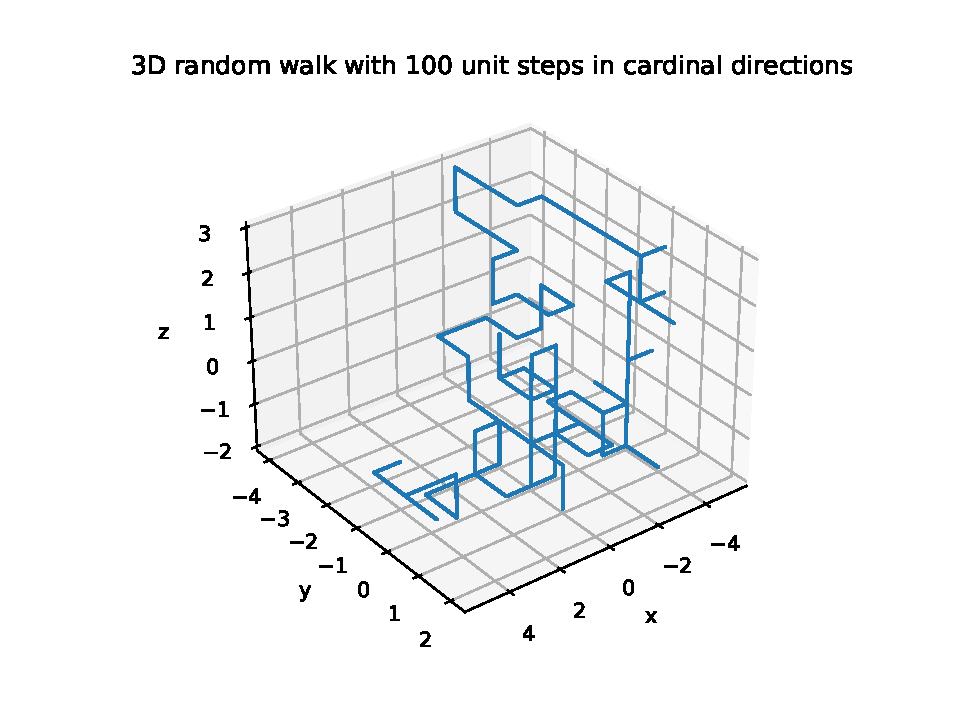
\includegraphics[width=\textwidth]{img/1-grid-100.pdf}
  \end{minipage}
  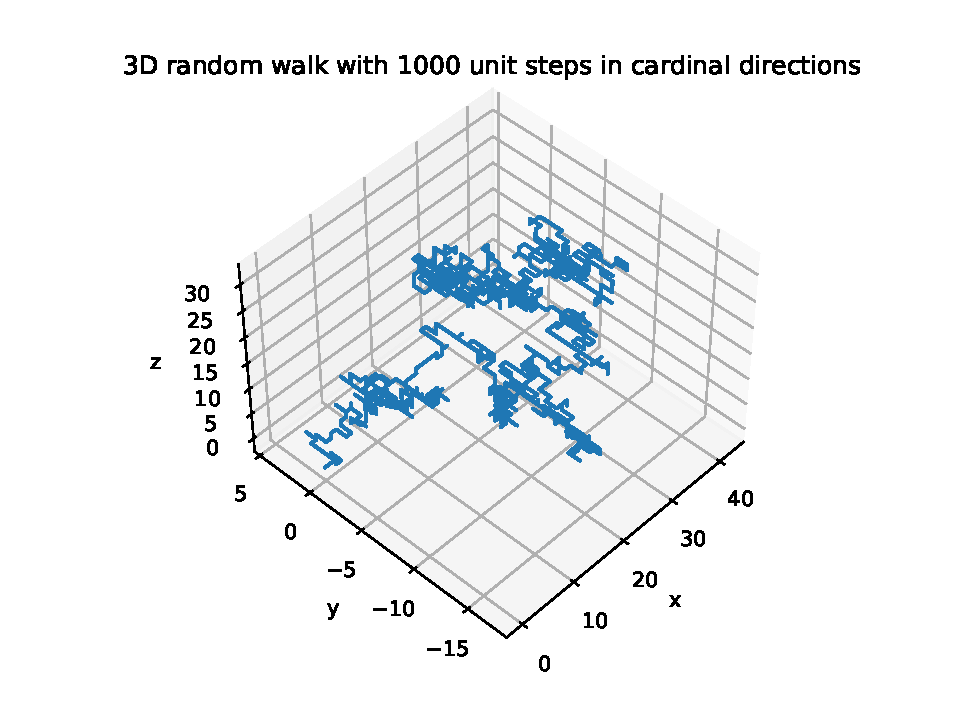
\includegraphics[scale=0.49]{img/1-grid-1000.pdf}
\end{figure}

It's immediately apparent that now there's much more room for the path to occupy since the path itself still
essentially is only one dimensional, yet we've added an additional dimension to work with. There's way less
overlap, especially looking at the case when the number of steps $N \geq 100$, compared to the same situation in
2D, shown both above and in Project 2.

Samples from the generated freely jointed chain paths (from here on out simply referred to as chain paths) looks
like the following.

\begin{figure}[!ht]
  \centering
  \begin{minipage}{0.49\textwidth}
    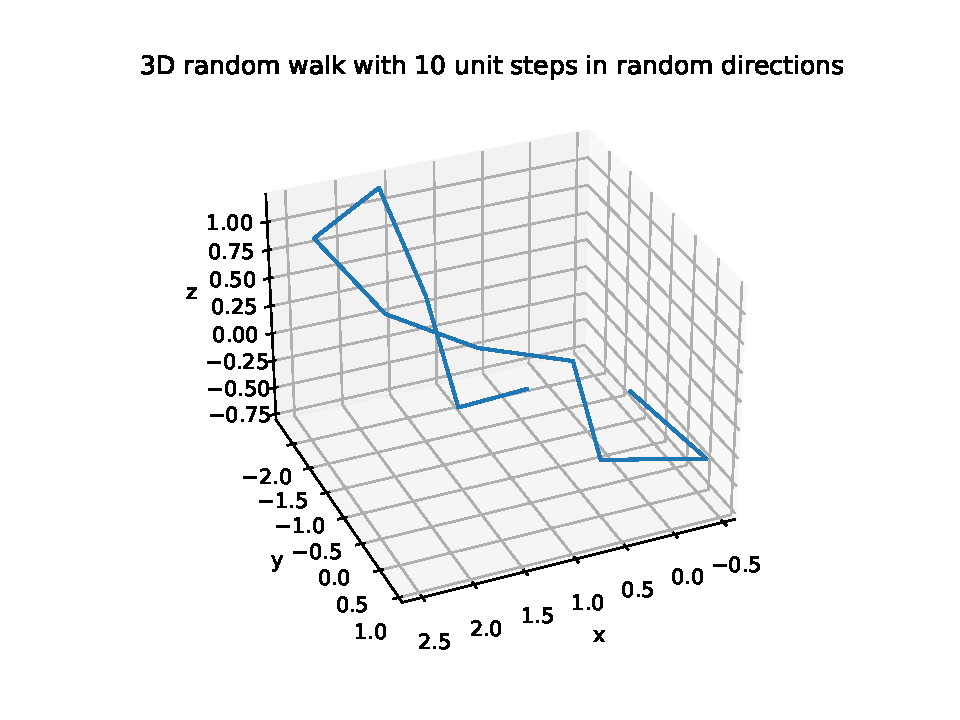
\includegraphics[width=\textwidth]{img/1-chain-10.pdf}
  \end{minipage}
  \begin{minipage}{0.49\textwidth}
    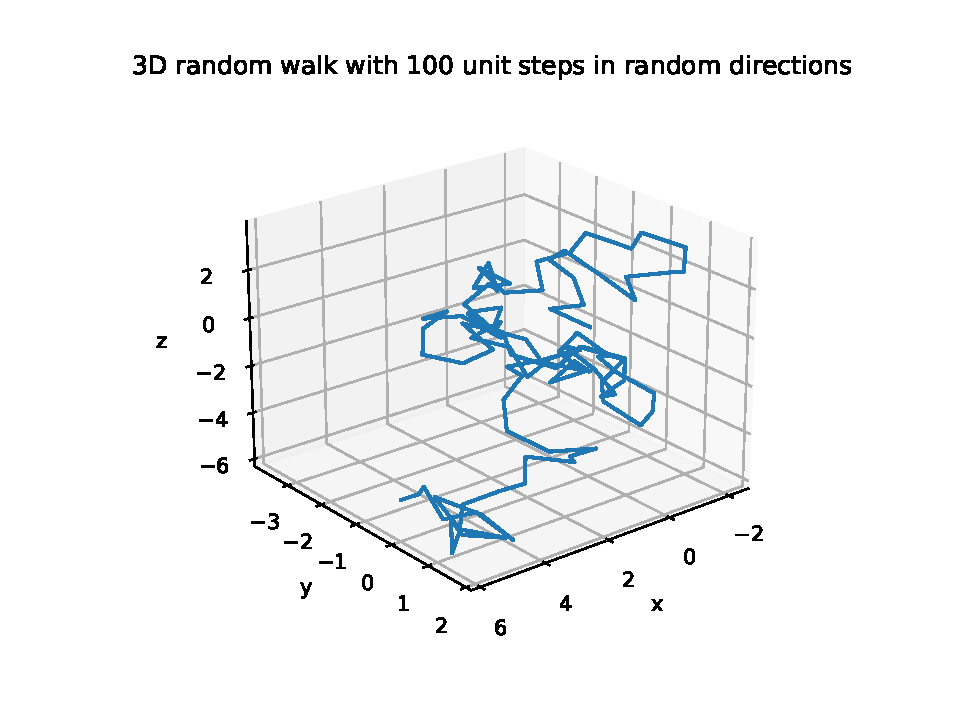
\includegraphics[width=\textwidth]{img/1-chain-100.pdf}
  \end{minipage}
  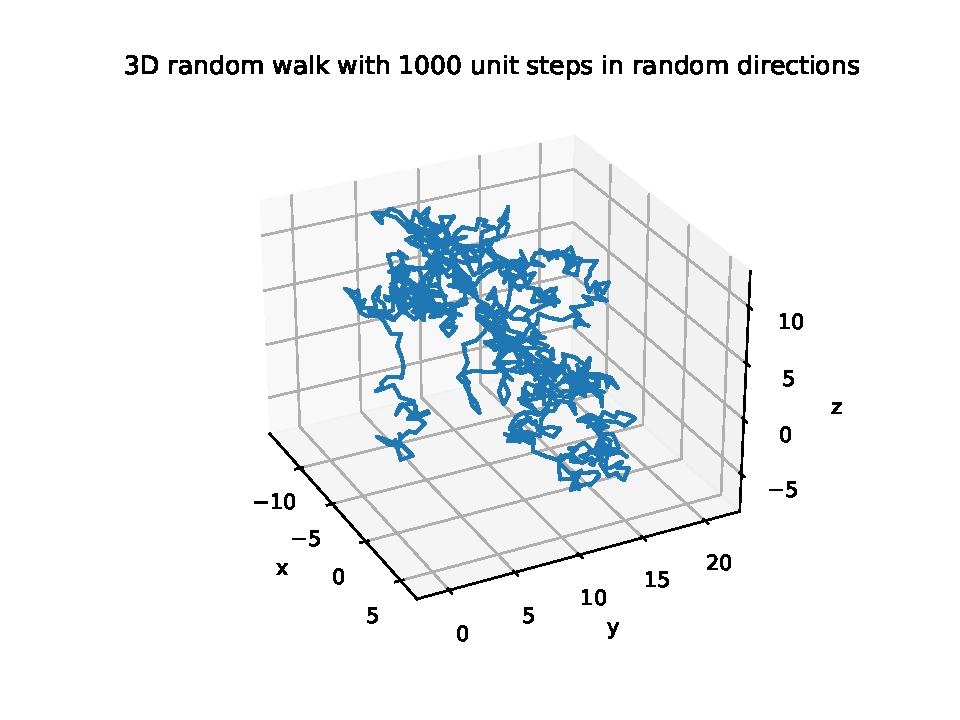
\includegraphics[scale=0.49]{img/1-chain-1000.pdf}
\end{figure}

\FloatBarrier

Compared to the grid walks, the chain walks are much more chaotic in nature. This can be quite easily explained
though, due to the fact that the orthogonal lines in the grid walk provide order, which is something the chain
walks lack. At a glance, the chain walks look more organic compared to the grid walks, but it's purely a visual
conclusion with no statistical evidence to back it up.

\section*{Analysis}

We can use the Root Mean Squared end-to-end Distance ($\mathrm{D}_{RMS}$, also abbreviated as RMSD in this report)
and Root Mean Squared Fluctuation (RMSF) of the distance to more precisely measure the qualities of the walks.
Given $M$ samples of a quantity $R$ (in this case, $R$ is the end-to-end distance the walk covers), we can compute
the following:

\begin{itemize}
  \item The variance $V$:
  \begin{equation*}
    V = \left\langle R^2 \right\rangle - \left\langle R \right\rangle ^2
  \end{equation*}
  Here $\left\langle \cdot \right\rangle$ denoting the average of something.

  \item The Root Mean Squared Distance $\mathrm{D}_{RMS}$ or RMSD:
  \begin{equation*}
    \mathrm{D}_{RMS} = \sqrt{\frac{1}{M}\sum_{i = 1}^{M} R_i^2} = \sqrt{\left\langle R^2 \right\rangle}
  \end{equation*}

  \item An estimate of the Root Mean Squared Fluctuation RMSF:
  \begin{equation*}
    \mathrm{RMSF} \approx \sqrt{V \, \frac{M}{M - 1}}
  \end{equation*}

  \item As well as the Standard Error Estimate SEE:
  \begin{equation*}
    \mathrm{SEE} \approx \sqrt{\frac{V}{M - 1}} = \frac{\mathrm{RMSF}}{\sqrt{M}}
  \end{equation*}
\end{itemize}

See the lecture notes for Project 2 for additional information. \cite{Hess}
With $R^2 = x^2 + y^2 + z^2$, we can plot the RMSD and RMSF for both types of walks. Starting with the 3D grid
walk:

\begin{figure}[!ht]
  \centering
  \begin{minipage}{0.49\textwidth}
    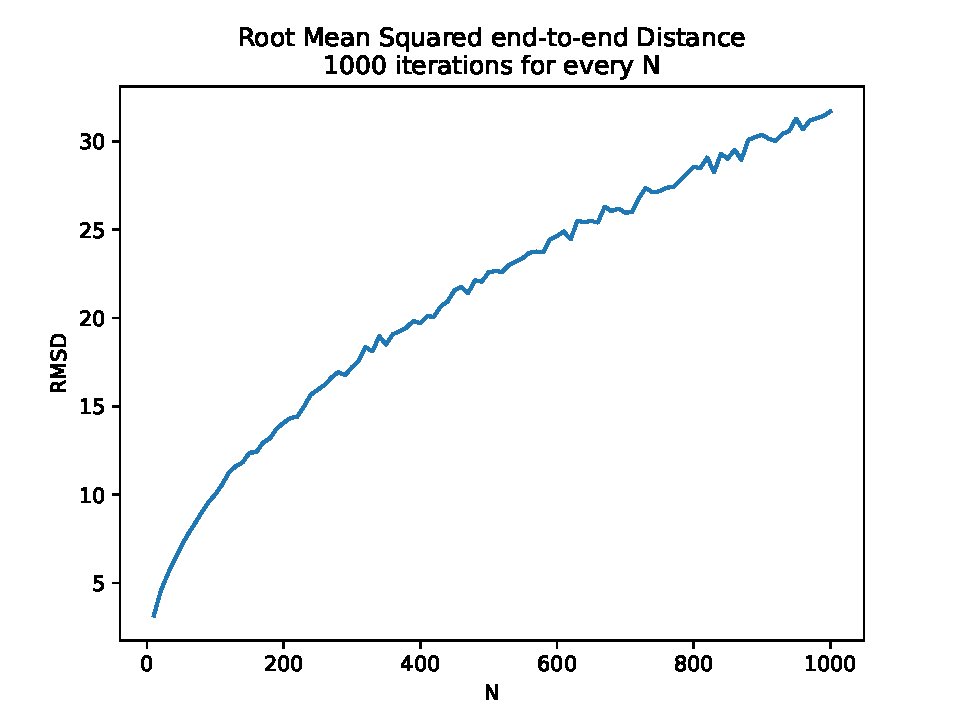
\includegraphics[width=\textwidth]{img/2-grid-rmsd.pdf}
  \end{minipage}
  \begin{minipage}{0.49\textwidth}
    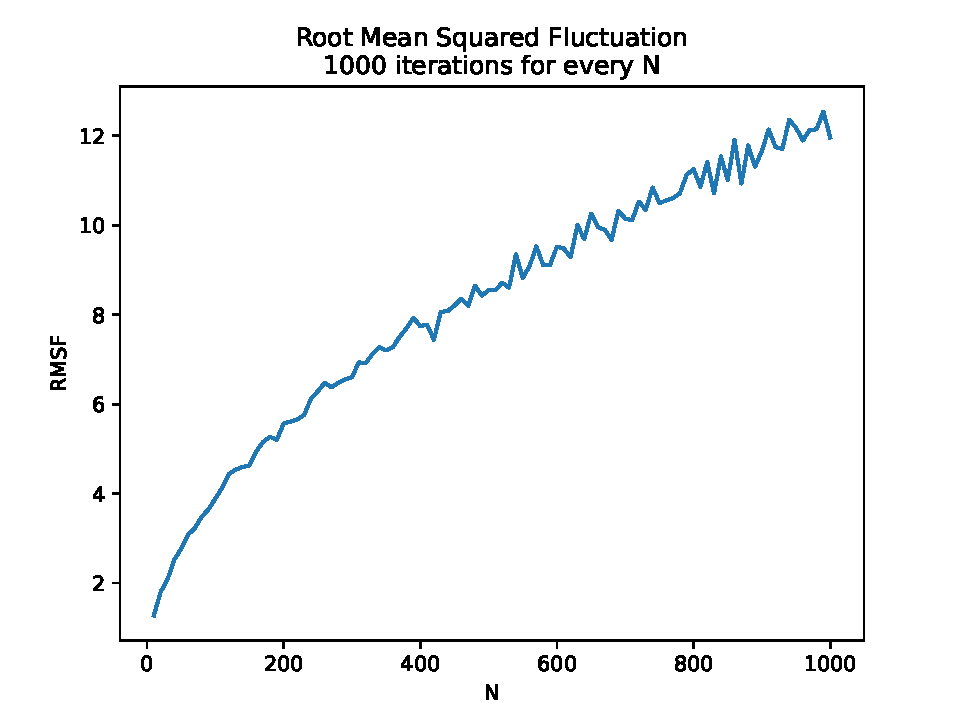
\includegraphics[width=\textwidth]{img/2-grid-rmsf.pdf}
  \end{minipage}
\end{figure}

For reference, here are the same graphs but for two dimensions, taken from Project 2:

\begin{figure}[!ht]
  \centering
  \begin{minipage}{0.49\textwidth}
    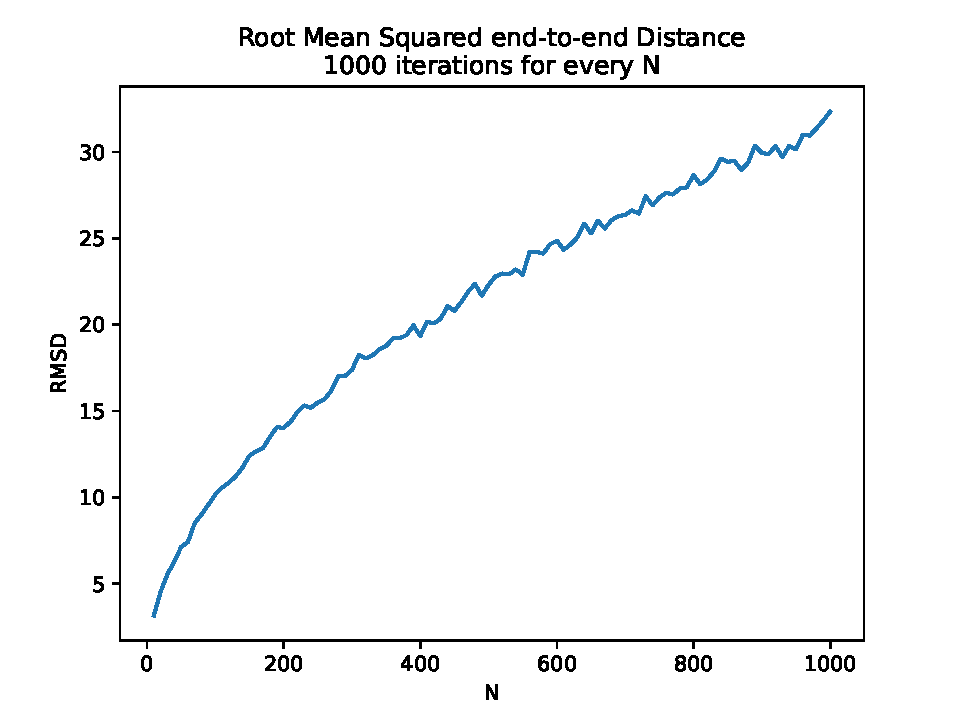
\includegraphics[width=\textwidth]{img/2-grid-2d-rmsd.pdf}
  \end{minipage}
  \begin{minipage}{0.49\textwidth}
    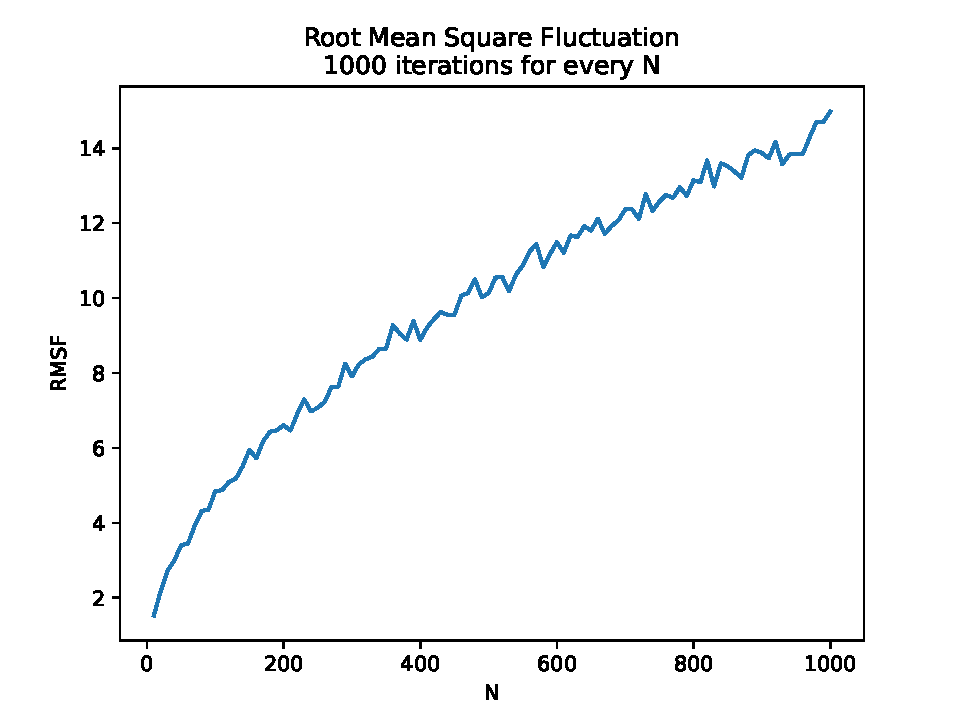
\includegraphics[width=\textwidth]{img/2-grid-2d-rmsf.pdf}
  \end{minipage}
\end{figure}

We notice that both cases are \emph{surprisingly} similar to each other. $\mathrm{D}_{RMS}$ appears to grow at
about exactly the same pace regardless of if we're working in two or three dimensions. What might be even more
surprising though is that we seem to obtain a lower fluctuation in the distance covered when we add the 3rd
dimension. Now, plotting the same metrics for the chain walks, we obtain the following graphs:

\begin{figure}[!ht]
  \centering
  \begin{minipage}{0.49\textwidth}
    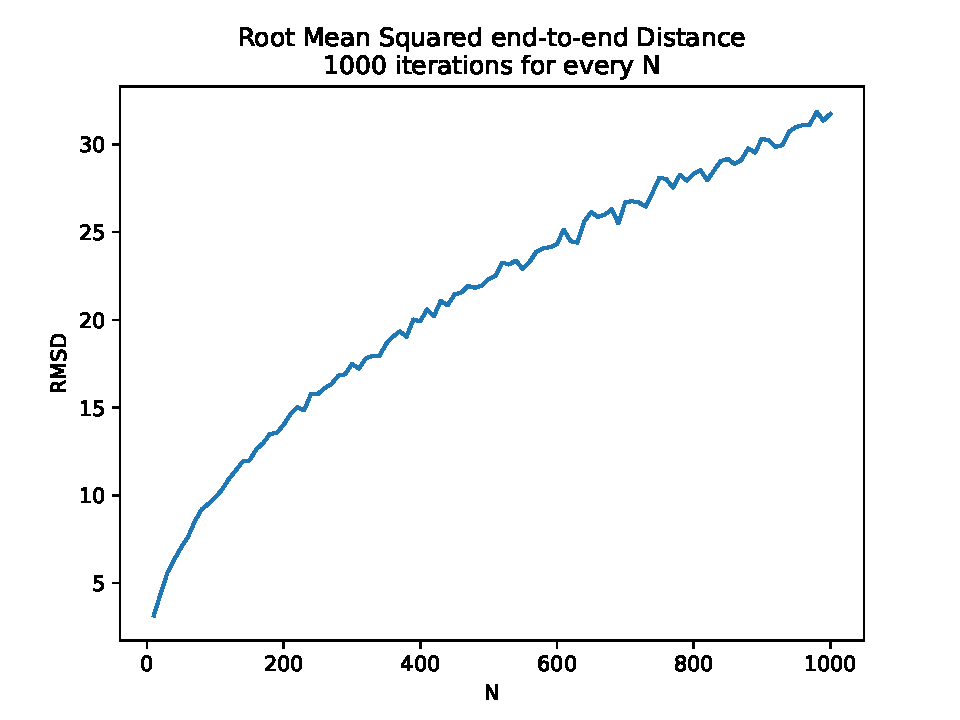
\includegraphics[width=\textwidth]{img/2-chain-rmsd.pdf}
  \end{minipage}
  \begin{minipage}{0.49\textwidth}
    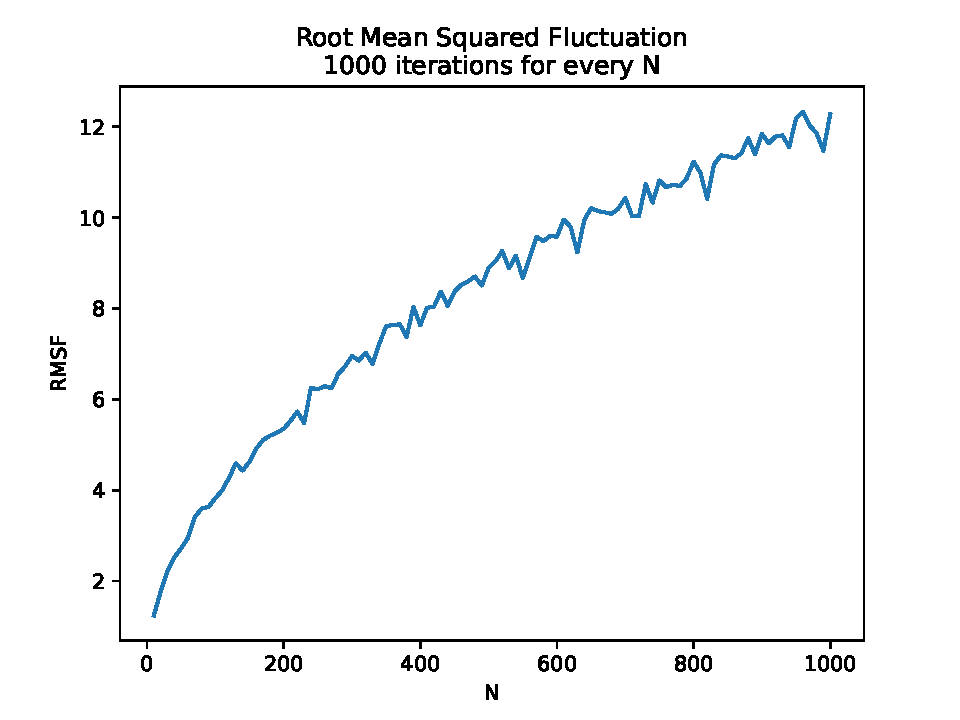
\includegraphics[width=\textwidth]{img/2-chain-rmsf.pdf}
  \end{minipage}
\end{figure}

\FloatBarrier

This was the more surprising part. The distance reached by the random walk as a freely jointed chain reaches is
almost identical to the distance reached by the grid walk. Not only that, but the fluctuation of said distance is
essentially the same too. The small difference between the results can likely be attributed to the fact that only
$1000$ random walks were done per value of $N$, so it's bound to have some discrepancies. In general though, this
suggests that there's no meaningful difference between the two types of walks in regards to the distance reached.

\section*{Self Avoiding Walks}

While a three-dimensional random walk might resemble a real polymer better (at least visually), polymers in the
real world still cannot cross themselves, since that would require two atoms occupying the same point in space.
This can be addressed by making the random walk \emph{self avoiding}. To implement a self avoiding random walk in
a simple fashion, any generated random walk that would self intersect will be discarded.

\subsection*{Theory}

Transforming a random walk into a self avoiding walk is simple enough: store all points that's been visited already
and discard the walk if any point is encountered twice.

\subsubsection*{Grid Walk}

One slight optimization can be made though: since we know that any walk which
immediately backtracks on itself will get discarded, we can prevent this option from being available to the
randomizer when selecting where to step next. However, we \emph{do not} check if the walk is about to step to a
point which has already been visited before, since that would remove possibilities for where to take the next step,
and thus the walk would no longer be truly random.

\subsubsection*{Chain Walk}

A chain walk will by default essentially never visit the same space twice simply because of how it's implemented.
In practice though, atoms (and by extension polymers) do take up physical space and aren't just zero dimensional
points. To simulate this with the random walk, we can assign spheres with a given radius to each point that's been
visited, and only allow steps for which the new sphere will not make contact with any other sphere. For a walk with
step length $1$, the maximum radius possible is $0.5$, since any radius larger than that will make the spheres
intersect no matter where the step is taken.

\subsection*{Application}

Generating walks and discarding them as soon as they self-intersect means the success rate (i.e., the fraction of
walks that successfully generate without visiting a point twice compared to the total amount of generated walks)
will decrease as the length of the generated walk increases. Plotting this relation for the grid walk, both normally
but also with a logarithmic scale on the y axis, yields the following graphs. Do note the flat part of the plot in
the beginning, which implies that the basic algorithm to prevent the walk from instantly backtracking works.

\begin{figure}[!ht]
  \centering
  \begin{minipage}{0.49\textwidth}
    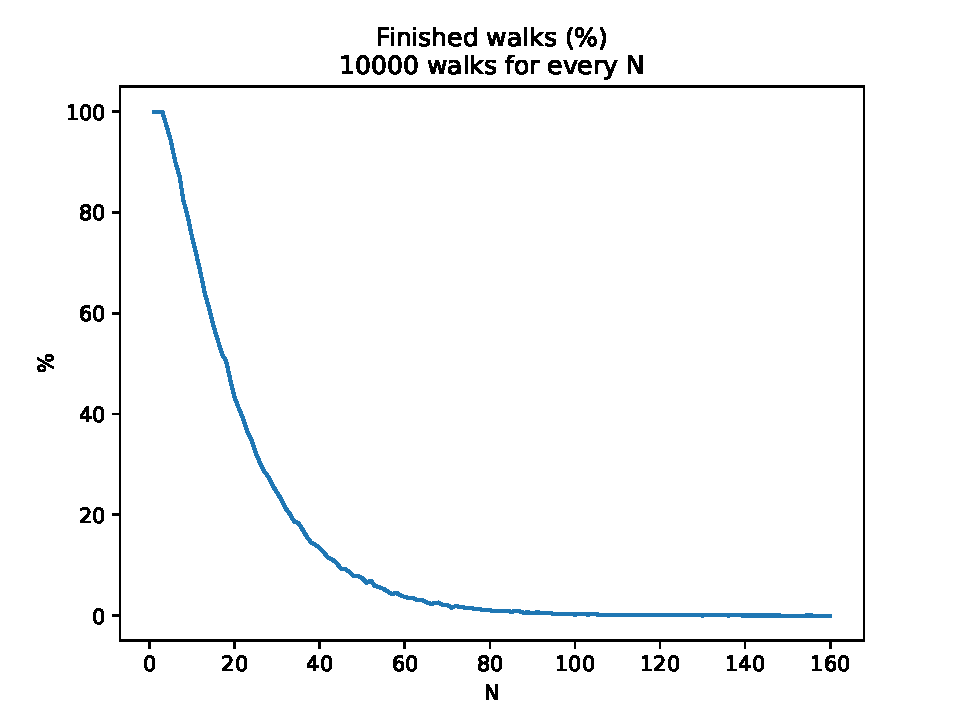
\includegraphics[width=\textwidth]{img/3-grid-fraction-finished.pdf}
  \end{minipage}
  \begin{minipage}{0.49\textwidth}
    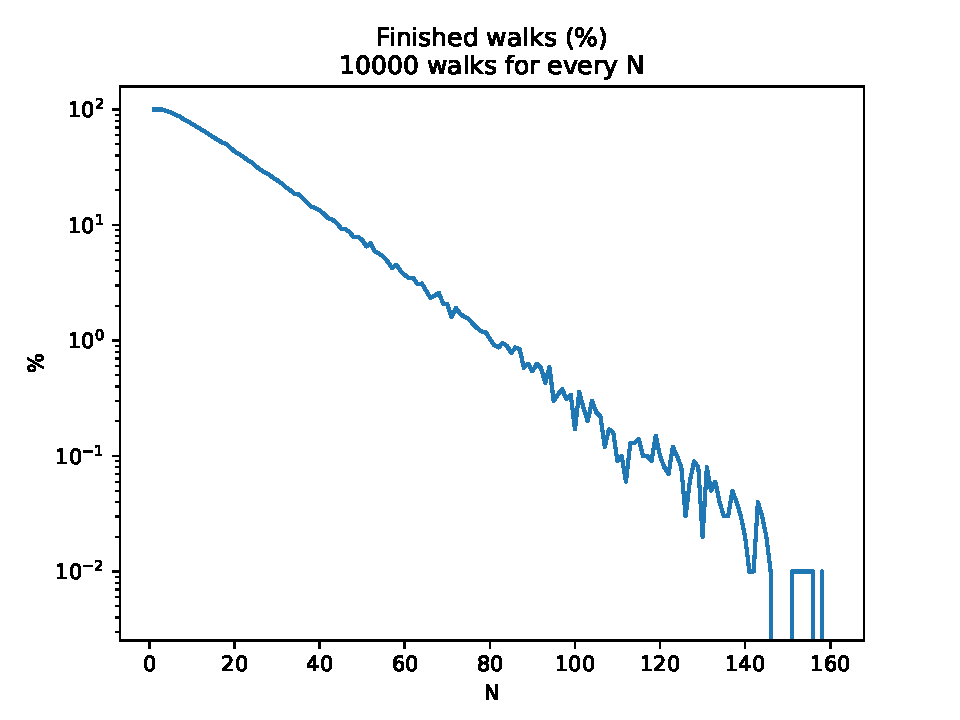
\includegraphics[width=\textwidth]{img/3-grid-fraction-finished-log.pdf}
  \end{minipage}
\end{figure}

We can here generate walks of much longer length and still have a decent success rate. It's only when
$N \approx 120$ that the success rate drops below $0.1\%$. This can be compared to the success rate of the
two-dimensional case, where it only took $N \approx 35$ for the success rate to drop below $0.1\%$ (see Project 2).
Now, repeating the same process for the chain walk with different values of the sphere radius (recall that $0.5$ is
the maximum possible value) and plotting the results yields the following two graphs.

\begin{figure}[!ht]
  \centering
  \begin{minipage}{0.49\textwidth}
    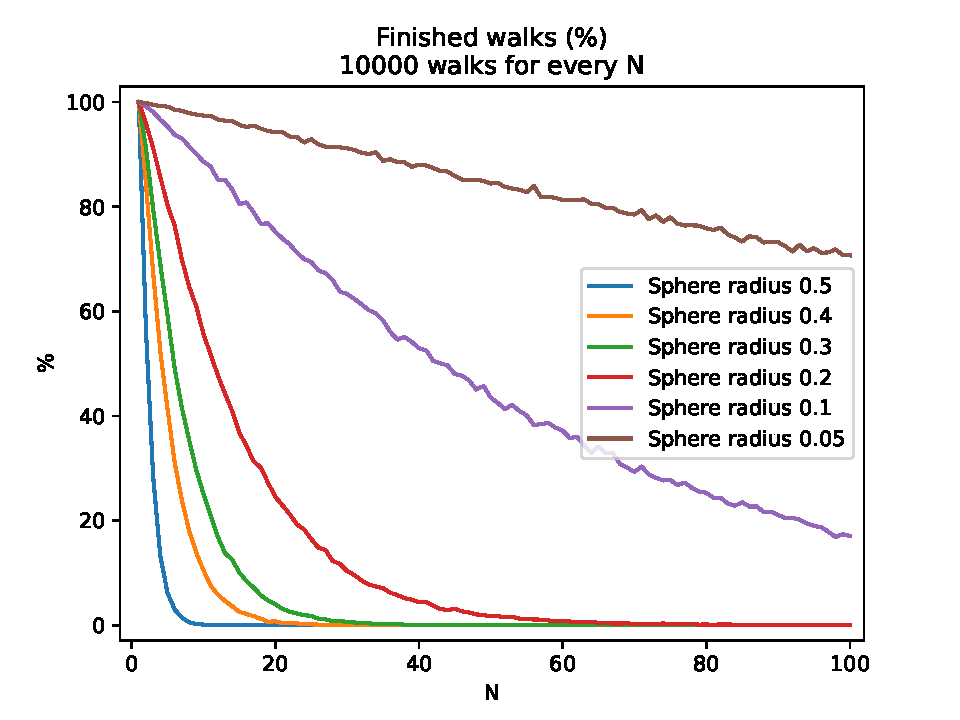
\includegraphics[width=\textwidth]{img/3-chain-fraction-finished.pdf}
  \end{minipage}
  \begin{minipage}{0.49\textwidth}
    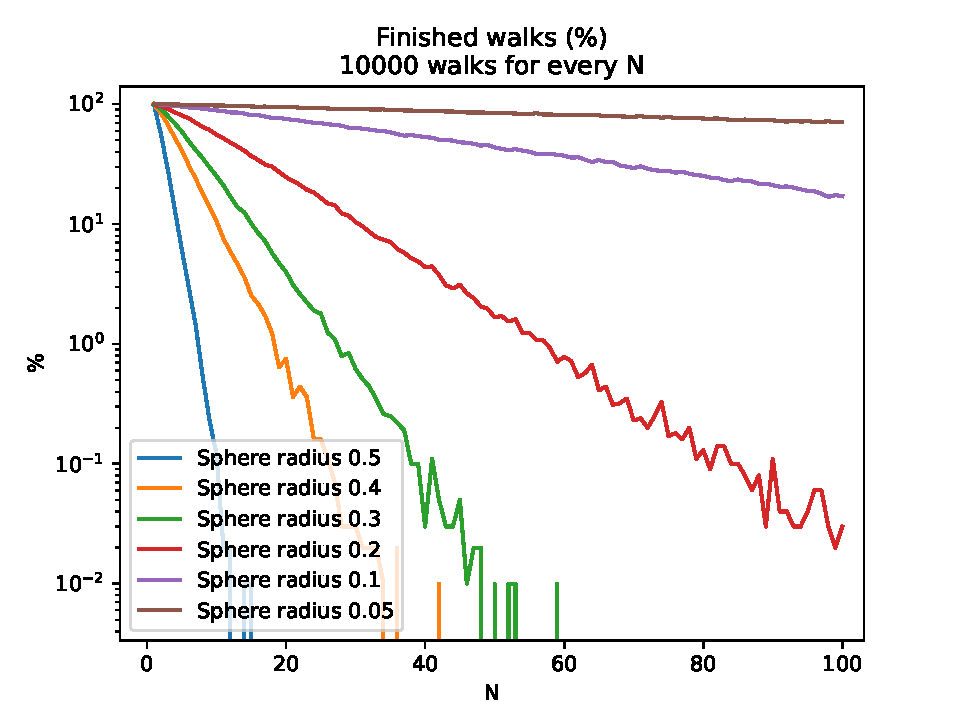
\includegraphics[width=\textwidth]{img/3-chain-fraction-finished-log.pdf}
  \end{minipage}
\end{figure}

This graph had to be cut short on the x axis due to the computation time quickly getting out of hand for smaller
values of the sphere radius. The running time for this algorithm is already $O(n^2)$ (or more precisely,
$\theta (n^2)$, with $O$ and $\theta$ here referring to Big O Notation) due to having to check against every other
stored point for every step, and the only thing that speeds it up in the beginning is that for large values of the
sphere radius, lots of walks immediately gets thrown out. We can note that the success rate decreases at roughly
at the same pace as the grid walk when the sphere radius is a little smller than $0.2$ (which gives a success rate
of about $10^{-\frac{1}{2}} \% \approx 0.31\%$ at $N = 100$). For simplicity's sake and for ease of comparison, we'd
ideally want to use one value only for the radius of the spheres attached to each point in the self avoiding chain
walk. Assuming the size of an atom is roughly $1$ Ångström and the distance between atoms in a molecule is "a few"
Ångströms, using a value of $0.2$ for the sphere radius doesn't seem entirely unreasonable.

\section*{Comparison}

\subsection*{Different Types Of Walks}

Computing $\mathrm{D}_{RMS}$ for all four types of walks (grid and chain, both normal and self avoiding) with a
sphere radius of $0.2$ for the self avoiding chain walk, for $N \in [1, 75]$ yields the following graphs.

\begin{figure}[!ht]
  \centering
  \begin{minipage}{0.49\textwidth}
    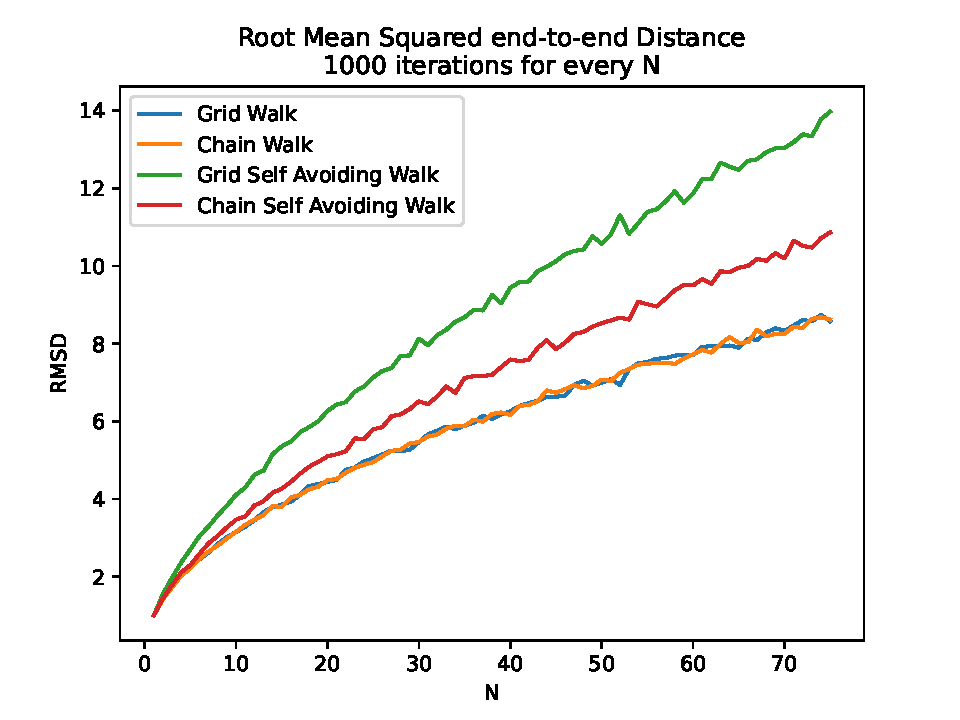
\includegraphics[width=\textwidth]{img/4-rmsd-comparison.pdf}
  \end{minipage}
  \begin{minipage}{0.49\textwidth}
    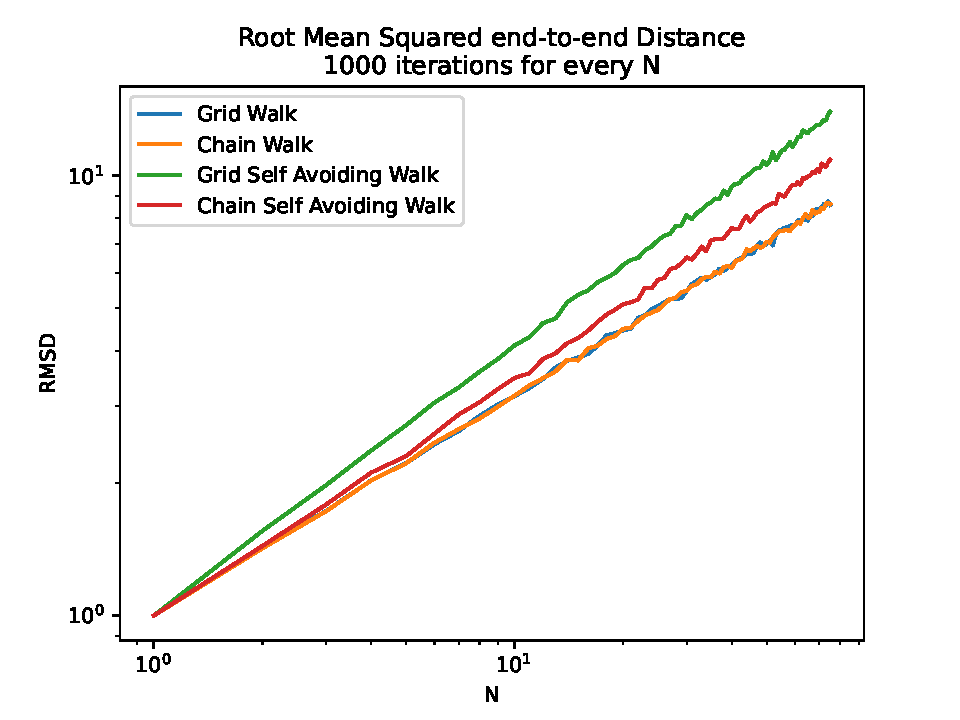
\includegraphics[width=\textwidth]{img/4-rmsd-comparison-loglog.pdf}
  \end{minipage}
\end{figure}

There's no substantial difference between the different types of random walks, however this does confirm the
conclusion that was drawn earlier; the non-self avoiding walks behave very similar to each other in terms of
distance reached. The self avoiding random walk on a grid reaches farther than any other walk per number of steps
taken, on average, since when having such limited options, most possible steps will either point away from the
origin or be more or less parallel to it (i.e., not taking the walk any further but not any closer to the origin
either). This is similar to the case for the self avoiding chain walk, where the possible steps point mostly away
from the origin too, albeit just a smaller fraction of the total, since the step can be taken in almost any direction
except for more or less straight backwards, due to the sphere at the point lastly visited. Lastly, for the non-self
avoiding walks, every step option is equally likely, so it makes sense seeing the $\mathrm{D}_{RMS}$ for these types
of walks slightly lower than the self avoiding walks.

\subsection*{RMSD Across Different Radii}

Finally, we'll compare $\mathrm{D}_{RMS}$ across different sphere radii. Due to the way the algorithm is designed,
at $N = 15$ when $r = 0.5$, the rate for a successful walk is already down to $10^{-2}$ to $10^{-3} \%$,
making successful walks exceedingly rare. The x axis thus had to be cut down a lot, in order for the computation time
to still remain manageable. Plotting $\mathrm{D}_{RMS}$ for different radii yields the following.

\begin{figure}[!ht]
  \centering
  \begin{minipage}{0.49\textwidth}
    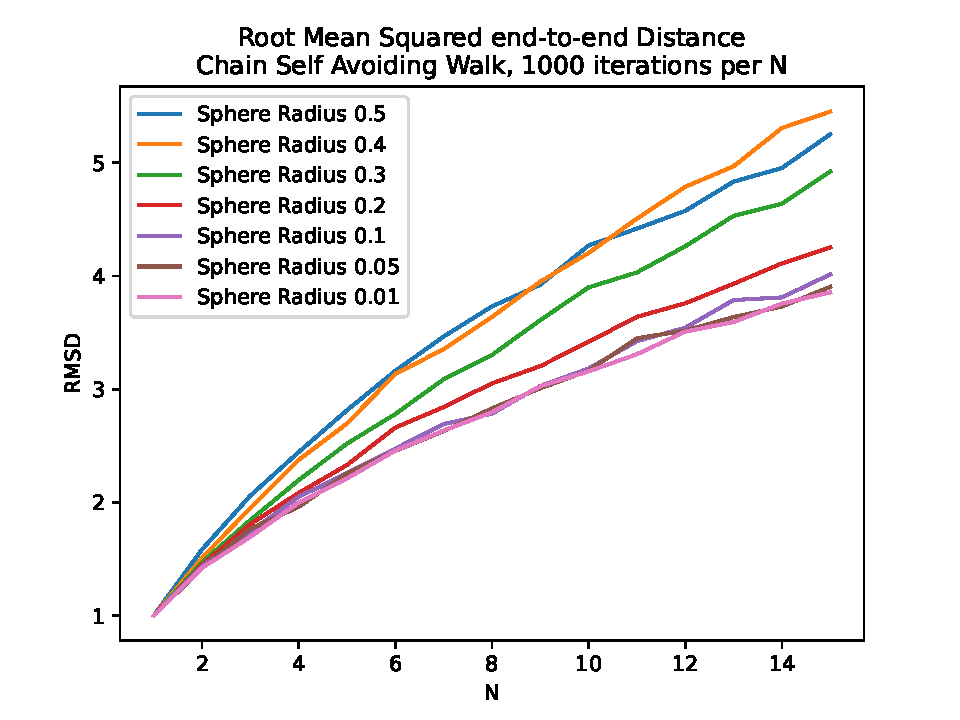
\includegraphics[width=\textwidth]{img/4-rmsd-radius-comparison.pdf}
  \end{minipage}
  \begin{minipage}{0.49\textwidth}
    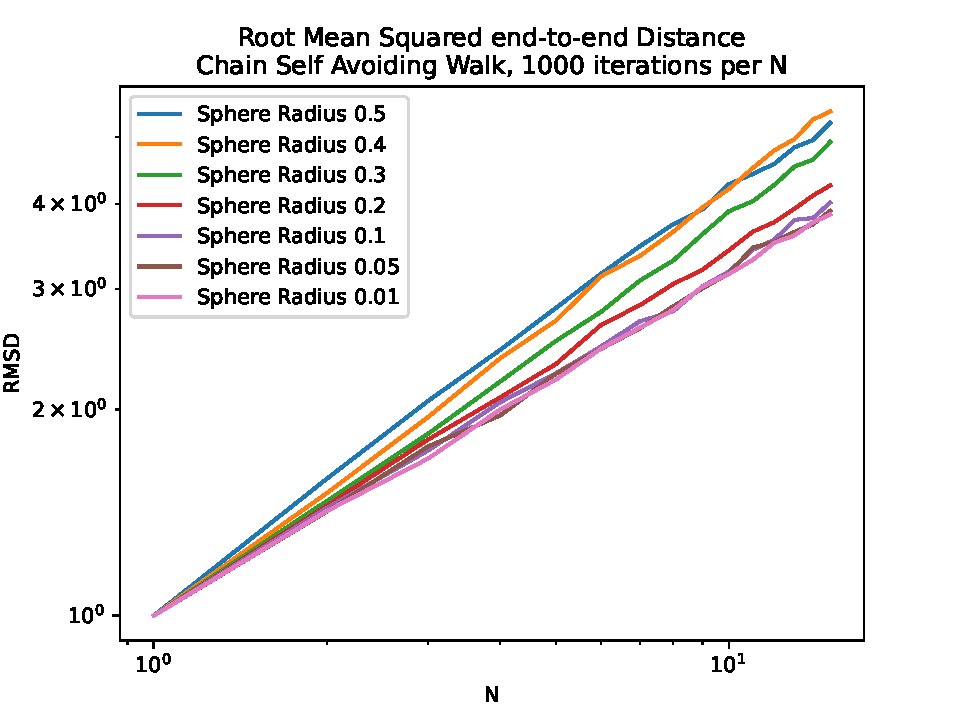
\includegraphics[width=\textwidth]{img/4-rmsd-radius-comparison-loglog.pdf}
  \end{minipage}
\end{figure}

What's apparent and not surprising is that $\mathrm{D}_{RMS}$ decreases slightly when the sphere radius does.
A smaller sphere radius means a smaller portion of possible valid steps lead away from the origin, meaning more
steps are taken in a backwards manner, at least compared to the walks with a bigger radius.

\begin{thebibliography}{9}
  \bibitem{MathWorld} Weisstein, Eric W. "Sphere Point Picking." From MathWorld -- A Wolfram Web Resource.
  https://mathworld.wolfram.com/SpherePointPicking.html

  \bibitem{Hess} Hess, Berk. "Random processes \& complex systems." Simulation and Modelling SI1336, 14 Nov. 2022,
  KTH. Lecture.
\end{thebibliography}

\end{document}